\documentclass{article}
\usepackage{amsmath}
\usepackage{amssymb}
\usepackage{geometry}
\usepackage{graphicx}
\usepackage{tikz}

\geometry{a4paper, margin=1in}

\title{Comprehensive Notes on Set Theory and Applications}
\author{Ahmed Sultan P}
\date{}

\begin{document}

\maketitle

\section{Fundamental Types of Sets}
A set is a well-defined collection of distinct objects. Understanding the classification of sets is foundational for higher mathematics and computer science.

\begin{itemize}
    \item \textbf{Cardinality of a set ($|A|$ or $n(A)$):} The total number of distinct elements contained within a set.
    \item \textbf{Finite set:} A set with a specific, countable number of elements where the counting process eventually terminates (e.g., the number of nodes in a fixed cluster).
    \item \textbf{Infinite set:} A set with an endless number of elements, where cardinality is not a natural number (e.g., the set of all integers, $\mathbb{Z}$).
    \item \textbf{Null set / Empty set ($\emptyset$ or $\{\}$):} A set containing zero elements. It is a fundamental property that the null set is a subset of every possible set.
    \item \textbf{Equal set ($A = B$):} Two sets are equal if they contain the exact same elements, regardless of order. Formally: 
    $$A = B \implies \forall x \in A \iff x \in B \implies A \subseteq B \text{ and } B \subseteq A$$
    \item \textbf{Equivalent set:} Two sets are equivalent if they share the same cardinality ($|A| = |B|$), even if the elements themselves differ.
    \item \textbf{Subset ($A \subseteq B$):} Set $A$ is a subset of $B$ if every element of $A$ is also contained in $B$. 
    $$A \subseteq B \implies \forall x \in A \implies x \in B$$
    \item \textbf{Proper Subset ($A \subset B$):} Set $A$ is a subset of $B$, but $A \neq B$. 
    \item \textbf{Superset:} If $A \subseteq B$, then $B$ is the superset of $A$, meaning $B$ fully encompasses $A$.
    \item \textbf{Universal set ($U$):} The overarching master set containing all objects, elements, and sets under consideration for a specific problem domain.
    \item \textbf{Power set ($\mathcal{P}(S)$):} The set containing all possible subsets of a given set $S$, including the null set and the set itself. If $|S| = n$, then $|\mathcal{P}(S)| = 2^n$.
    \item \textbf{Singleton set / Singular set:} A set containing exactly one element (cardinality of 1).
    \item \textbf{Countable set:} A set whose elements can be put into a one-to-one correspondence with the set of natural numbers (can be finite or countably infinite).
\end{itemize}
\newpage
\section{Core Set Operations}
Set operations allow us to combine and relate different sets. In backend engineering and relational database management systems (DBMS), these mathematical operations form the basis of relational algebra and SQL queries.

\begin{itemize}
    \item \textbf{Union ($A \cup B$):} The set of all elements that are in $A$, or in $B$, or in both.
    $$A \cup B = \{x \mid x \in A \text{ or } x \in B\}$$
    \textit{Application:} Corresponds to the \texttt{UNION} operator in SQL to combine the result sets of two or more \texttt{SELECT} statements.
    
    \item \textbf{Intersection ($A \cap B$):} The set of elements that are strictly common to both $A$ and $B$.
    $$A \cap B = \{x \mid x \in A \text{ and } x \in B\}$$
    \textit{Application:} Corresponds to the \texttt{INTERSECT} operator in relational databases, retrieving records present in both queried tables.
    
    \item \textbf{Set Difference ($A - B$ or $A \setminus B$):} The set of elements present in $A$ but completely absent from $B$.
    $$A - B = \{x \mid x \in A \text{ and } x \notin B\}$$
    \textit{Application:} Corresponds to the \texttt{EXCEPT} or \texttt{MINUS} operations in SQL.
    
    \item \textbf{Symmetric Difference ($A \Delta B$ or $A \oplus B$):} The set of elements in either $A$ or $B$, but crucially \textit{not} in their intersection.
    $$A \Delta B = (A - B) \cup (B - A)$$
    
    \item \textbf{Complement ($A^c$ or $A'$):} All elements in the Universal set $U$ that are not included in $A$.
    $$A^c = \{x \in U \mid x \notin A\} \implies A^c = U - A$$
    
    \item \textbf{Cartesian Product ($A \times B$):} The set of all possible ordered pairs where the first element is from $A$ and the second is from $B$.
    $$A \times B = \{(a, b) \mid a \in A, b \in B\}$$
    \textit{Application:} Forms the mathematical foundation for a \texttt{CROSS JOIN} in database routing and querying.
\end{itemize}

\section{Set Builder Notation Examples}
Set builder notation is a rigorous shorthand used to describe a set by stating the properties its members must satisfy.

\begin{enumerate}
    \item $A = \{x \in \mathbb{N} \mid x < 6\}$ \textit{(Natural numbers less than 6)}
    \item $B = \{x \in \mathbb{Z} \mid -2 < x < 2\}$ \textit{(Integers between -2 and 2 exclusively)}
    \item $C = \{x \mid x \text{ is a prime number and } x < 10\}$
    \item $D = \{x \mid x \text{ is a character in the string `ALGORITHM'}\}$
    \item $E = \{x \in \mathbb{R} \mid x^2 = 9\}$ \textit{(Real numbers whose square is 9)}
    \item $F = \{x \in \mathbb{N} \mid x \bmod 2 = 0 \text{ and } x < 10\}$ \textit{(Even natural numbers below 10)}
    \item $G = \{x \mid x \text{ is a day of the week starting with `S'}\}$
    \item $H = \{x \in \mathbb{Z} \mid x^2 < 10\}$ \textit{(Integers whose square is strictly less than 10)}
    \item $I = \{x \in \mathbb{N} \mid 12 \bmod x = 0\}$ \textit{(The set of all positive factors of 12)}
    \item $J = \{x \mid x \text{ is a vowel in the standard ASCII alphabet}\}$
\end{enumerate}

\section{Applications in Computer Science, AI \& Data Science}
Set theory translates directly into software architecture, data structures, and machine learning models. For instance, in object-oriented programming, data structures like \texttt{java.util.HashSet} strictly enforce mathematical set properties (namely, no duplicate elements) using hash codes.

\begin{itemize}
    \item \textbf{Universal Set \& Feature Space:} In AI, the Universal Set ($U$) often represents the complete $n$-dimensional feature space ($\mathbb{R}^n$). Every potential input vector is an element of this set.
    \item \textbf{Finite Set (Classification):} The target labels in a supervised classification problem form a finite set (e.g., $L = \{\text{Spam}, \text{Not Spam}\}$).
    \item \textbf{Infinite Set (Regression):} The output predictions of a neural network utilizing a linear activation function form an infinite set of real numbers ($\mathbb{R}$).
    \item \textbf{Subsets in Training Pipelines:} When partitioning a dataset, the training, validation, and testing sets are mutually exclusive proper subsets of the master dataset.
    \item \textbf{Null Set in Cleaning:} If a validation script searches for null pointers or missing values in a perfectly clean relational database table, the resulting query returns a Null Set ($\emptyset$).
\end{itemize}

\section{Hasse Diagrams (Visualizing Ordered Sets)}
A Hasse diagram is a simple way to draw a picture of a set where the elements have a specific hierarchy or order (like "less than" or "is a subset of"). 

Instead of drawing messy arrows everywhere, Hasse diagrams use three straightforward rules to keep the drawing clean:
\begin{enumerate}
    \item \textbf{Bottom-to-Top:} Smaller or "lower" elements are drawn at the bottom. Larger or "higher" elements are drawn above them.
    \item \textbf{Connecting Lines:} If element $x$ is directly below element $y$ in the hierarchy, draw a straight vertical or diagonal line connecting them. 
    \item \textbf{No Redundancy:} We never draw loops (an element connecting to itself), and we never draw skip-lines (if $x$ connects to $y$, and $y$ connects to $z$, we rely on that path and do not draw a redundant direct line from $x$ to $z$).
\end{enumerate}

\subsection*{Example 1: A Simple Linear Relation for $\{a, b\}$}
Imagine a set containing just two elements, $\{a, b\}$, and we are given a simple rule: $a \le b$ (read as "$a$ comes before $b$"). 
\begin{itemize}
    \item Since $a$ is smaller, it goes at the bottom.
    \item Since $b$ is larger, it goes at the top.
    \item We connect them with a single line.
\end{itemize}

\[
\begin{tikzpicture}
    \node (b) at (0,1) {$b$};
    \node (a) at (0,0) {$a$};

    \draw (b) -- (a);
\end{tikzpicture}
\]
\newpage
\subsection*{Example 2: The Power Set of $\{a, b\}$ (Subset Relation)}
A very common set theory exercise is drawing the Hasse diagram for the \textbf{subsets} of $\{a, b\}$. 
The power set (all subsets) is: $\mathcal{P} = \{\emptyset, \{a\}, \{b\}, \{a, b\}\}$. The hierarchy rule here is "is a subset of" ($\subseteq$).

\begin{itemize}
    \item \textbf{Bottom level:} The empty set ($\emptyset$) is a subset of everything, so it sits at the very bottom.
    \item \textbf{Middle level:} The singleton sets $\{a\}$ and $\{b\}$ both contain one element. $\emptyset$ is a subset of both, so lines go up from $\emptyset$ to $\{a\}$ and $\{b\}$. However, neither $\{a\}$ nor $\{b\}$ is a subset of the other, so they sit side-by-side with no line connecting them horizontally.
    \item \textbf{Top level:} The full set $\{a, b\}$ contains everything. Lines go up from $\{a\}$ and $\{b\}$ to $\{a, b\}$ at the very top.
\end{itemize}

\[
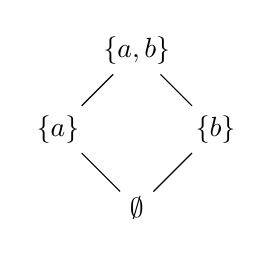
\begin{tikzpicture}
\node (ab) at (0,2) {$\{a,b\}$};
\node (a)  at (-1,1) {$\{a\}$};
\node (b)  at (1,1) {$\{b\}$};
\node (e)  at (0,0) {$\emptyset$};

\draw (ab) -- (a);
\draw (ab) -- (b);
\draw (a) -- (e);
\draw (b) -- (e);
\end{tikzpicture}
\]

\end{document}